\newpage
\section{Load System}
The purpose of this block is to measure the electrical current generated by the Generator in order to control the amount of power delivered to a load.

Due to the complexity of the Load System it's design, implementation and unit test is split according to the IBD below. It should be noted that the Load and the Super Capacitor is located on the Load-plate which is separated from the remaining system.

\begin{figure}[H]
	\centering
	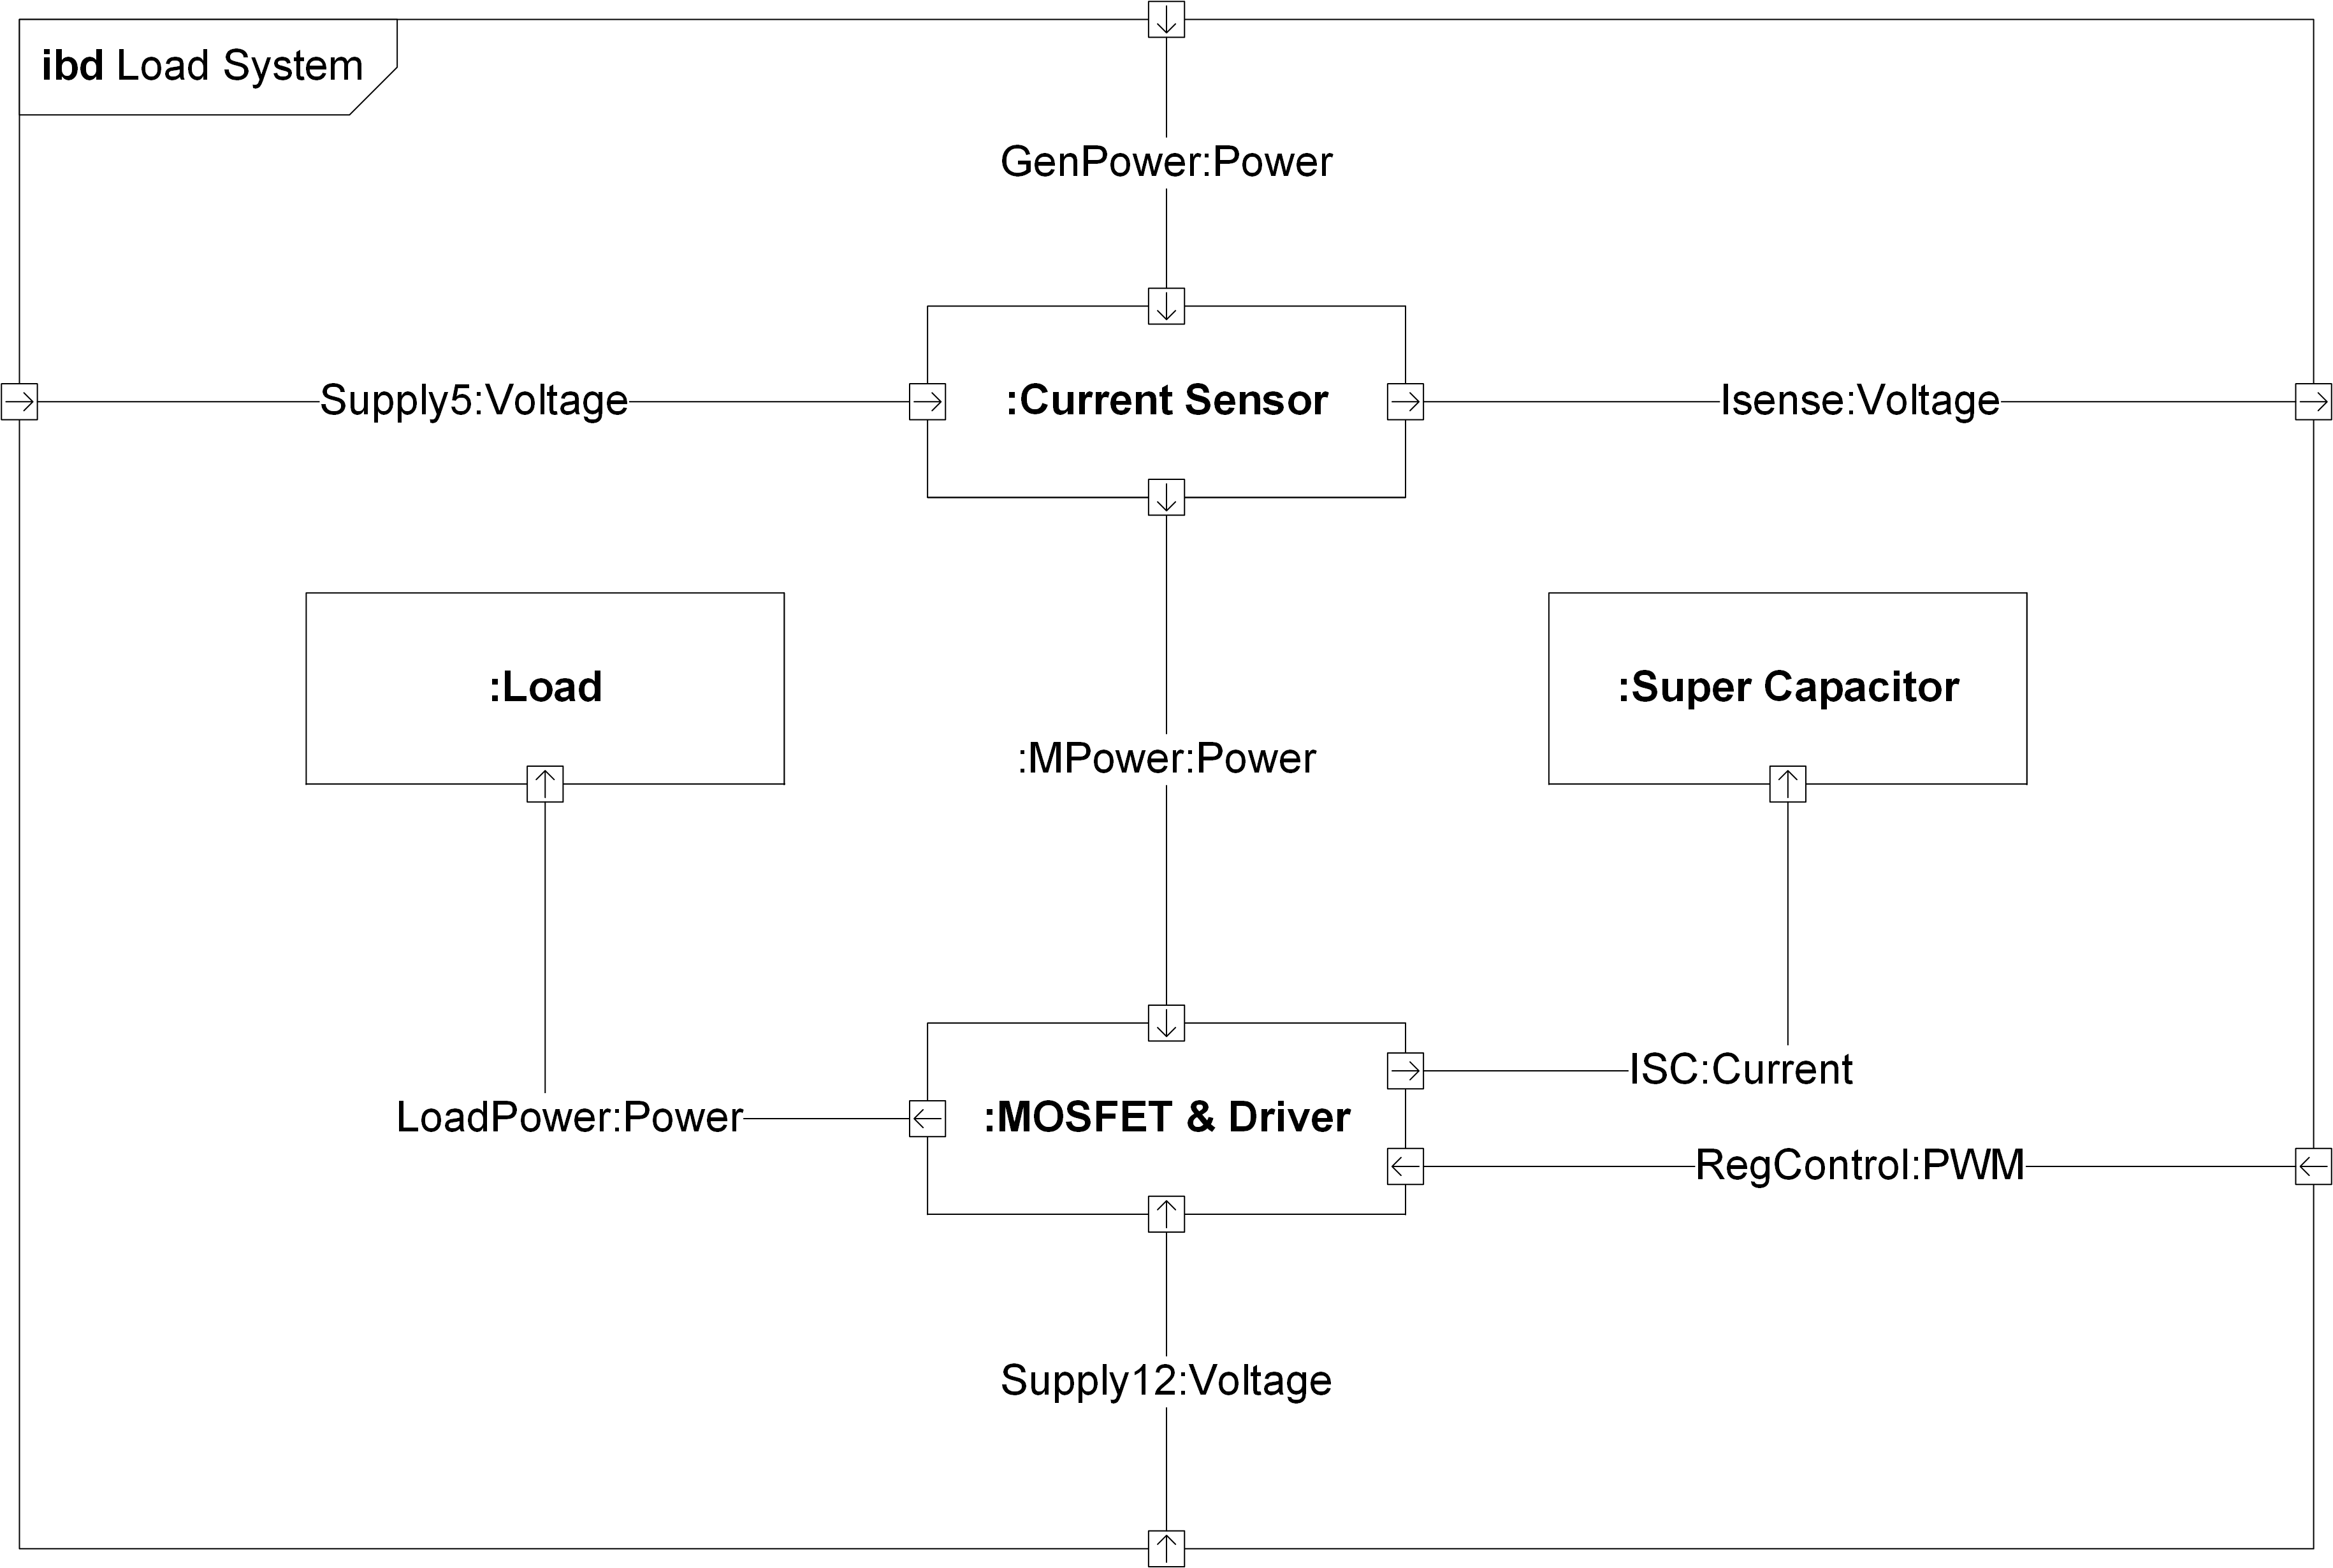
\includegraphics[width=1\linewidth]{Hardware/Pictures/IBD_LoadSystem}
	\caption{IBD of the Load System}
	\label{fig:IBD_Load_System}
\end{figure}

A short explanation for each subsystem seen in the Load System's IBD is given below. A more detailed explanation for each subsystem is given in the subsequent sections.
\begin{itemize}
	\item \textbf{Load}\\
	A passive load which converts generated electrical energy to thermic energy (heat).
	\item \textbf{Current Sensor}\\
	A current transducer which measures the current produced by the Generator's generated voltage in order to control the system using a PID-controller.
	\item \textbf{Super Capacitor}\\
	A capacitor which will counter the inductive reactance of the Generator in order to prevent current-transients.
	\item \textbf{MOSFET \& Driver}\\
	A power MOSFET (and an associated MOSFET-driver) which controls the amount of current delivered to the Load.
\end{itemize}
\newpage

\subsection{Analysis}
\label{sec:LoadSystemAnalysis}
The amount of power delivered to the Load can be controlled using a MOSFET which is turned on and off by a PWM-signal. The PWM-signal can be regulated such that the average current through the MOSFET during one period can be used to calculate the power delivered to the load. The power can be calculated as:
\begin{equation}
	P_{load} = V \cdot I = R_{load} \cdot I^2
\end{equation}
The current delivered to the Load R\textsubscript{load} should be measured using the Current Sensor. This leads to the simple draft of the system containing the Generator, the MOSFET, the controlling PWM-signal and the Load which can be seen on Figure \ref{fig:Load_System} below.

\begin{figure}[H]
	\centering
	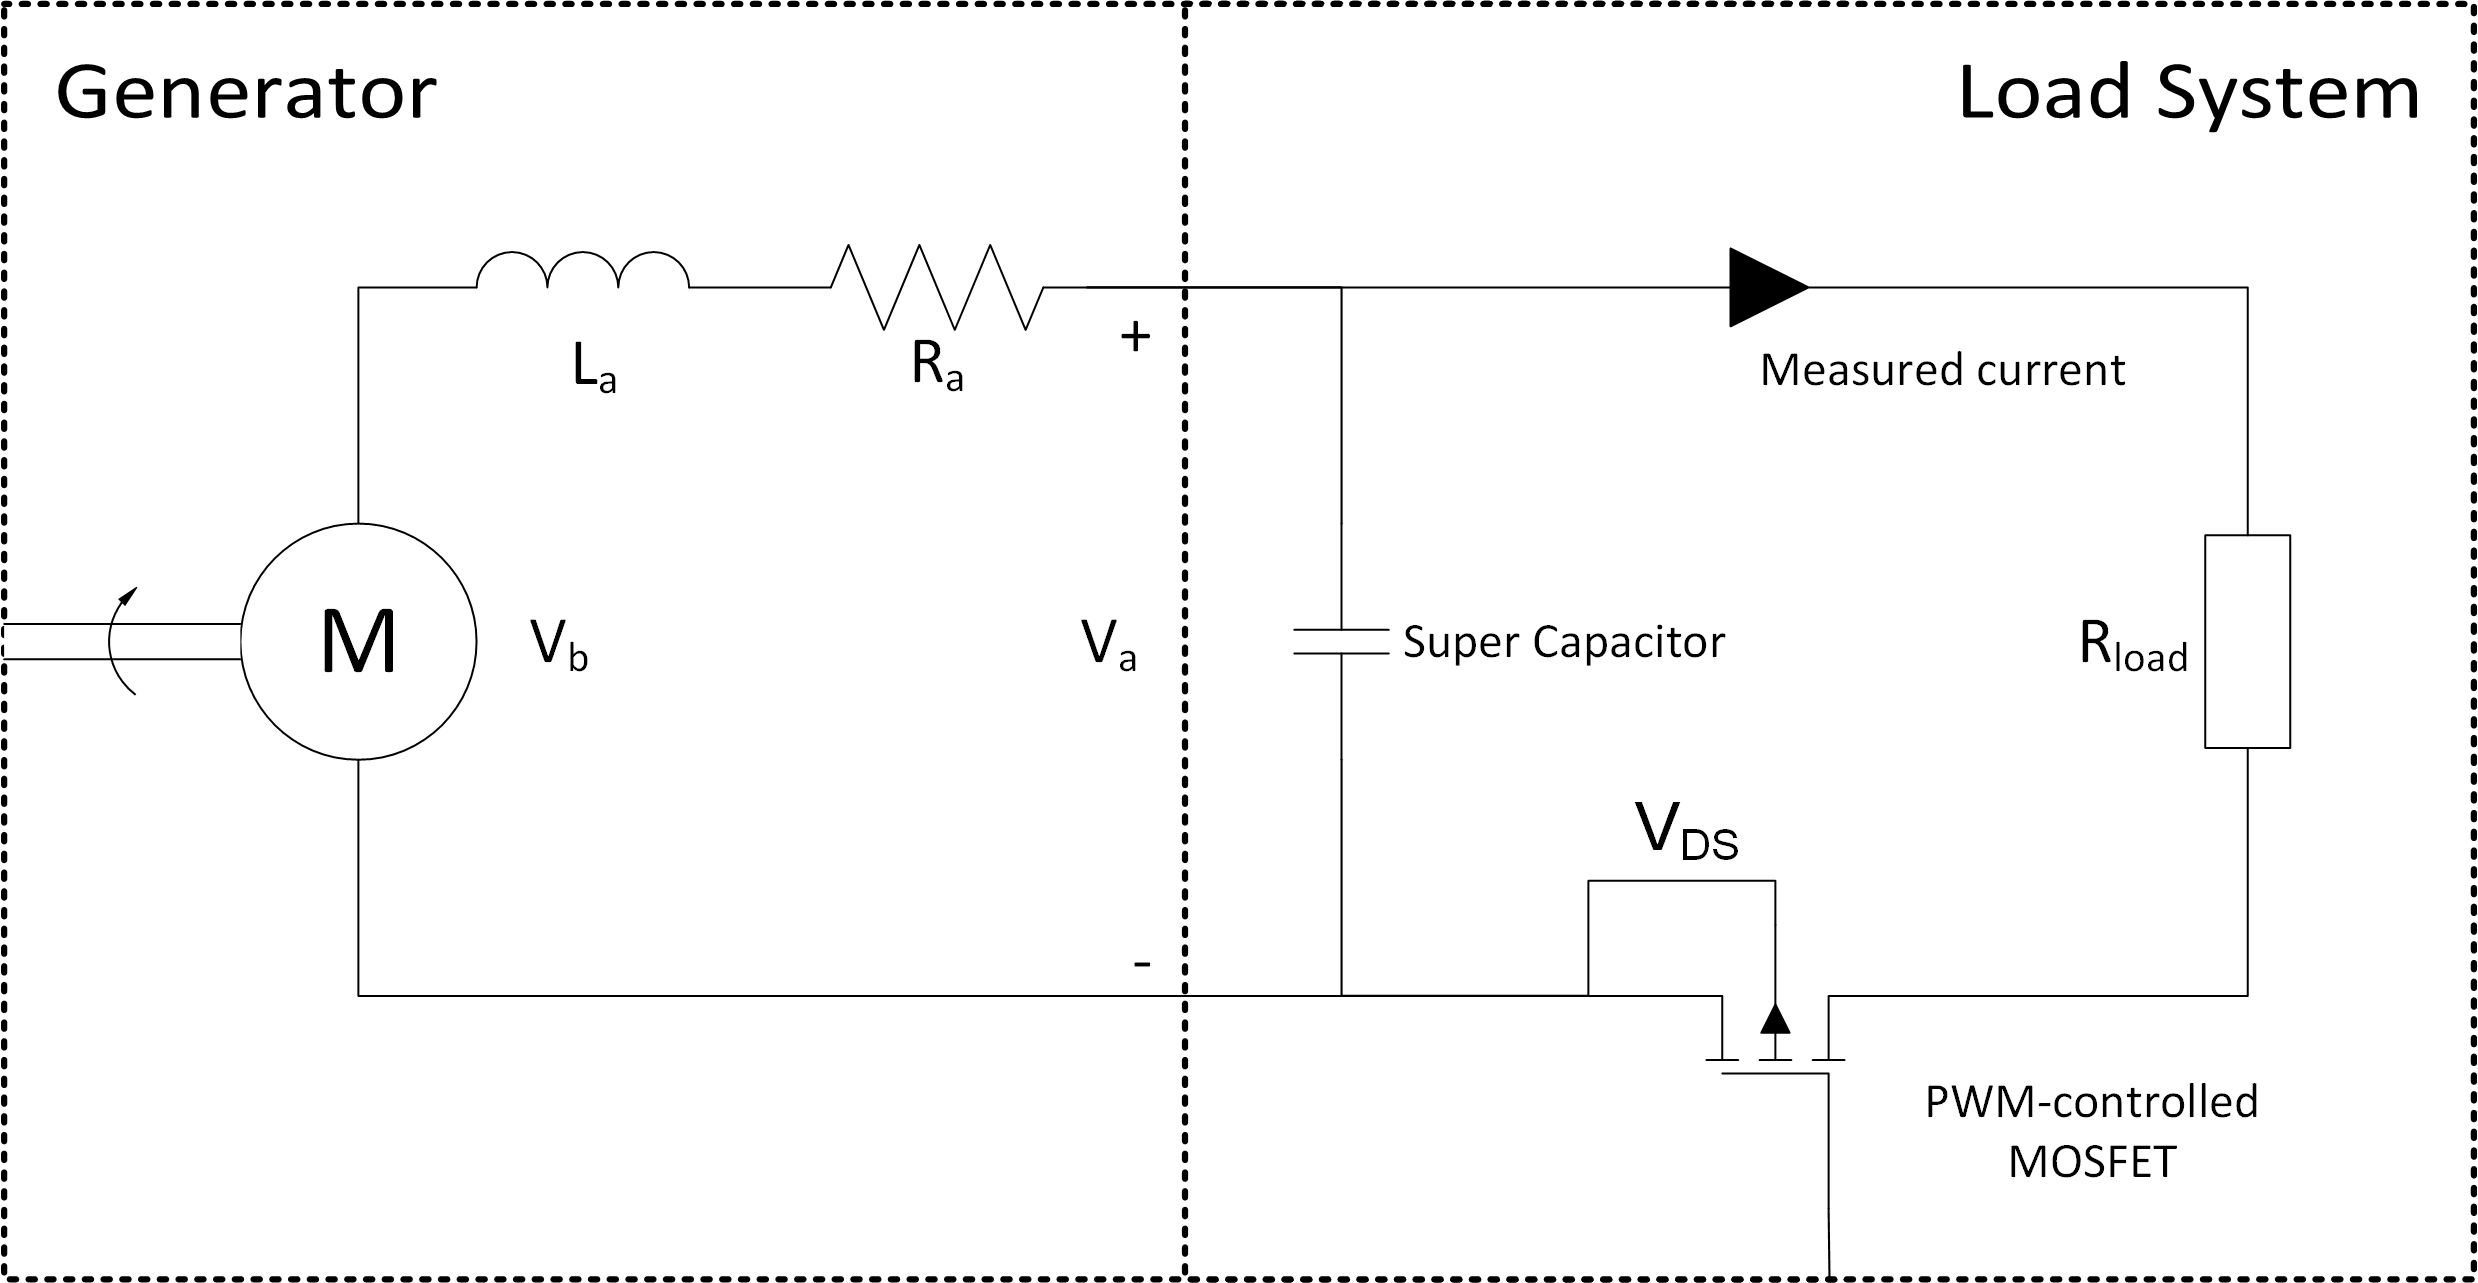
\includegraphics[width=0.7\linewidth]{Hardware/Pictures/LoadSystem}
	\caption{Connection between Generator and Load System}
	\label{fig:Load_System}
\end{figure}

It is assumed that the DC-generator's internal armature can be modelled using a voltage source in series with an inductor and a resistor. The voltage generated by the armature V\textsubscript{b} is proportional to the Generator's rotational velocity. The generated voltage over the armature's resistor will cause a current to flow.

This means that if the Generator's rotational speed is exposed to a  sudden change it will produce a large voltage-drop over the armature's inductor. This voltage will depend on the armature's inductance L\textsubscript{a} and can be calculated as:
\begin{equation}
	V_{La} = L_a \cdot \frac{di}{dt}
\end{equation}
Thus resulting in the fact that a very sudden change in rotational speed could cause a damaging voltage to be produced. This is not desirable and the inductive reactance should therefore be countered by a capacitative reactance. This is done by the Super Capacitor in parallel with the Generator.
\subsection{Current Sensor}
The Current Sensor must measure the current from the Generator in order to protect the Load System from electrical overload. The Current Sensor is built using a Hall-effect based current transducer of the type LTS 15-NP\cite{CurrentTransducer}. This type of transducer was also used in the Power Sensor design. Like before, the transducer is configured in such a way that it is able to measure currents up to $\SI{48}{\ampere}$ with a accuracy of 0.2\%.

The Current Sensor is able to measure currents in the range of $\pm \SI{48}{\ampere}$. This range is simply chosen out of simplicity since this was the same as earlier. This range is bigger than what it must be as a $\SI{15}{\ampere}$ fuse is implemented in series with the sensor.

\begin{figure}[H]
	\centering
	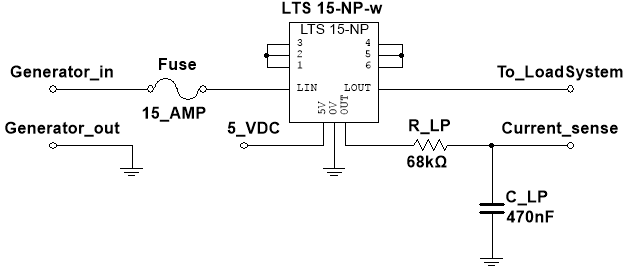
\includegraphics[width=0.8\linewidth]{Hardware/LoadSystem/CurrentSensor}
	\caption{Configuration of Current Sensor in the system}
	\label{fig:CurrentSensorCircuit}
\end{figure}

As the transducer is tested during the Power Sensor's unity test in section \vref{sec:PowerSensorTest}. During this test it was found that the output-volt can be calculated exactly as it is specified in the datasheet:
\begin{equation}
	V_{out} = 2.5 + \left( 0.625 \cdot \frac{I_{in}}{\SI{15}{\ampere}}\right)
\end{equation}
\subsection{MOSFET and Driver}
A MOSFET (Metal-Oxide-Semiconductor Field-Effect-Transistor) is used to control the amount of power which is delivered to the Load. The MOSFET must be able to handle a big amount of current produced by the Generator (\SI{44}{\ampere}).

The chosen transistor is a IRFP260N power MOSFET. This is an N-type MOSFET and is rated to be able to handle a drain-current I\textsubscript{D} of \SI{50}{\ampere} and a drain-source-voltage V\textsubscript{DSS} of \SI{200}{\volt}. Furthermore it is specified to have a very low on-resistance of \SI{40}{\milli \ohm} and can operate up to a temperature of \SI{175}{\celsius}.

A MOSFET-driver is needed in order to fully control the MOSFET's gate. The driver is needed to amplify the input-signal as:
\begin{itemize}
	\item The MOSFET's gate has a capacitive reactance which means that the gate must be charged before the MOSFET can conduct current. The charging-process would be extremely slow if it was done by the PSoC and the gate-current must be amplified in order to speed up the process.
	\item The MOSFET operates with a gate-source-voltage of \SI{12}{\volt}. This cannot be supplied by the PSoC and the gate-voltage must be amplified. 
\end{itemize}

In order to calculate the amount of current which is needed to charge the gate, the specified values for the Total Gate Charge Q\textsubscript{g} and the rise-time t\textsubscript{r} are found in the MOSFET's datasheet. These values are specified as:
\begin{equation}
\begin{split}
	Q_g &= \SI{234}{\nano \coulomb}\\
	t_r &= \SI{60}{\nano \second}
\end{split}
\end{equation}
Assuming a constant value the required gate-current can then be calculated as:
\begin{equation}
	I_{gate} = \frac{Q_g}{t_r} = \frac{\SI{234}{\nano \coulomb}}{\SI{60}{\nano \second}} = \SI{3.9}{\ampere}
\end{equation}
The chosen driver is a MCP1407 High Speed Power Driver. This driver is specified to be able to handle a large output-current of \SI{6}{\ampere} and can supply the MOSFET with \SI{12}{\volt}. It shold also be able to charge and discharge the MOSFET's gate in about \SI{40}{\nano \second}.

\begin{figure}[H]
	\centering
	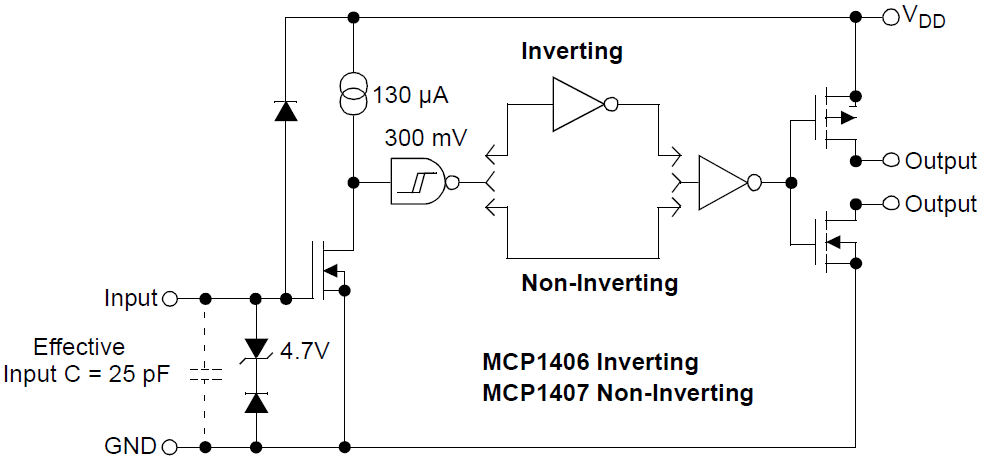
\includegraphics[width=0.7\linewidth]{Hardware/LoadSystem/GateDriver}
	\caption{MCP1407 High Speed Power Driver internal circuit}
	\label{fig:MOSFETDriverInternal}
\end{figure}

The MOSFET-driver is configured such that the outputs are connected with the MOSFET's gate through a \SI{3.3}{\ohm} resistor and the input is connected with the PSoC's output. The driver's positive supply line V\textsubscript{CC} is connected with the 12 VDC line in parallel with a \SI{1}{\micro \farad} and a \SI{0.1}{\micro \farad} capacitor. The driver's remaining pins are connected to ground as specified in the datasheet. The implemented design is seen below.

\begin{figure}[H]
	\centering
	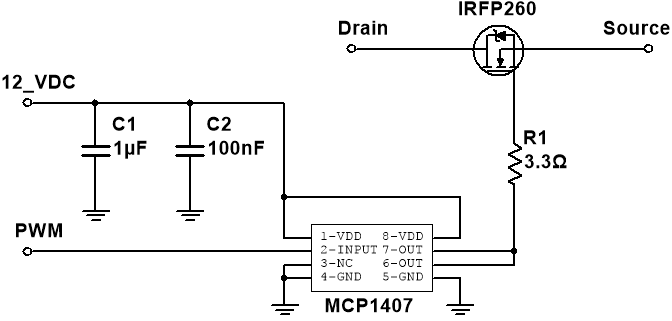
\includegraphics[width=0.7\linewidth]{Hardware/LoadSystem/MOSFET}
	\caption{Configuration of MOSFET and driver in the system}
	\label{fig:MOSFETCircuit}
\end{figure}
\subsection{Snubber}
Due to the fast-switching application of the MOSFET it will create transients which must be supressed. This can be done using an electrical snubber connected between the MOSFET's drain and source.
\subsection{Load}
The Load serves no other function than converting generated electrical energy to thermic energy (heat). This is done by using power resistors.\\
But then this is saying it impotent to choose the right setup.\\

\large List of things that has to be in order before using the load system!
\begin{itemize}
	\item {Generator}
	\subitem \textit{Must not exceed the power limit.}
	\subitem \textit{Must not exceed the speed limit.}
	\subitem \textit{the power limit must be greater or match the Test objects Power usage.}
	\item {Load resistor}
	\subitem \textit{Must not exceed the power limit with a voltage equal the nominal voltage.}
\end{itemize}

To get all these thing in order, some math has to been made. \\
First step is to find all information about the load systems components: 

\lstset{language=MATLAB}
\begin{lstlisting}
%% Constants

R_a             = 0.103;           % Anchor resistance (Ohm)
R_load          = 2.2;             % Load resistor (Ohm)
Kt              = 38.5*10^(-3);    % Torque Constant (Nm/A)
Gear            = 4.3;             % Gearing ratio in the motor (gg)
RR_r            = 0.076;           % RollingRoad radius (m)
Kb_rpm          = 248;             % Speed constant (rpm/V)
Kb              = Kt;              % Speed constant (rad/V)
AU2_peak_speed  = 30;              % AU2 peak speed (km/h)
V_N             = 24;              % Nominal Voltage (V)

%% limits

Generator_max_speed     = 9500;     %(rpm)
MAX_Continuous_current  = 10.8;     %(A)
Max_watt                = 200;      %(W)
R_load_max_watt         = 250;      %(W)
\end{lstlisting}

Note: There has been made a script that automatic calculate the best setup. (LoadSystem.m)\fxnote{mangler reference}\\
\\

The next step is to see how fast the Rolling Road is gonna rotate, then a test object are on it. In this example the test object is AU2. Then done the question is. Are there a need for gear-set to get a better rotating speed to generate a voltage what is closer to the nominal voltage?

\lstset{language=MATLAB}
\begin{lstlisting}
%% Calculation
% First is to find out what speed the generator is running.

% Rollings road max rotating speed (rpm)
RR_max_speed = AU2_peak_speed * KmToRpm 

% Voltage generated by the generator
% without gear
RR_Vb_nogear_max    = RR_max_speed * Kb_rpm^-1
% with gear
RR_Vb_gear_max      = RR_max_speed * Gear * Kb_rpm^-1
\end{lstlisting}

The result from this part is:

\begin{equation}
\begin{split}
	RR_{max_{speed}} = \SI{1047}{rpm}\\
	RR_{Vb_{nogear_max}} = \SI{4.22}{\volt}\\
	RR_{Vb_{gear_max}} = \SI{18.15}{\volt}
\end{split}
\end{equation}

It is clear. Gear option is the best option because it is closer to the nominal voltage.\\

The next step is to find out the best setup of the power resistor. With some calculation the best result is using two power resistor parallel. 

\lstset{language=MATLAB}
\begin{lstlisting}
% find the optimal resistor load setup.

Load_setup = [(R_load^2)/(R_load*2)+R_a, Max_watt*2; R_load+R_a, Max_watt; R_load*2+R_a, Max_watt*2];

best = 1;
for i = [1:length(Load_setup)]
if (RR_Vb_max^2 / Load_setup(i,1) <= Max_watt) && (Load_setup(i,2) > RR_Vb_max^2 / Load_setup(best,1)) && (RR_Vb_max^2 / Load_setup(i,1) > RR_Vb_max^2 / Load_setup(best,1))
best = i; 
end
end

Load_setup(best,1)
Power_max = RR_Vb_max^2 / Load_setup(best,1)
I_max = RR_Vb_max / Load_setup(best,1)
\end{lstlisting}


\begin{equation}
	\begin{split}
		R_{load} = \SI{1.203}{\Omega}\\
		Power_{max} = \SI{273.98}{\watt}\\
		I_{max} = \SI{15.09}{A}
	\end{split}
\end{equation}

Have to notify that this is not possible because it will cause a melt down of the Rolling Road.\\
That will result in max use of $ 73 \% $ then it runs at top speed!\\

After the limitation and calculate with $ Power_{max} = \SI{200}{\watt} $. The max torque, force and current can be calculated.

\lstset{language=MATLAB}
\begin{lstlisting}
% max torque, force and current.

I_max = (Power_max/RR_Vb_max)

torque_generator = (Power_max/RR_Vb_max) * Kt

if gear
torque_max = (Power_max/RR_Vb_max) * Kt * Gear
force_max = torque_max / RR_r
else
torque_max = (Power_max/RR_Vb_max) * Kt
force_max = torque_max / RR_r
end
\end{lstlisting}

The last results:

\begin{equation}
\begin{split}
Power_{max} = \SI{200}{\watt}\\
I_{max} = \SI{11.02}{A}\\
torque_{generator} = \SI{0.42}{\newton \metre}\\
torque_{max} = \SI{1.82}{\newton \metre}\\
force_{max} = \SI{24.00}{\newton}
\end{split}
\end{equation}

\begin{figure}[H]
	\centering
	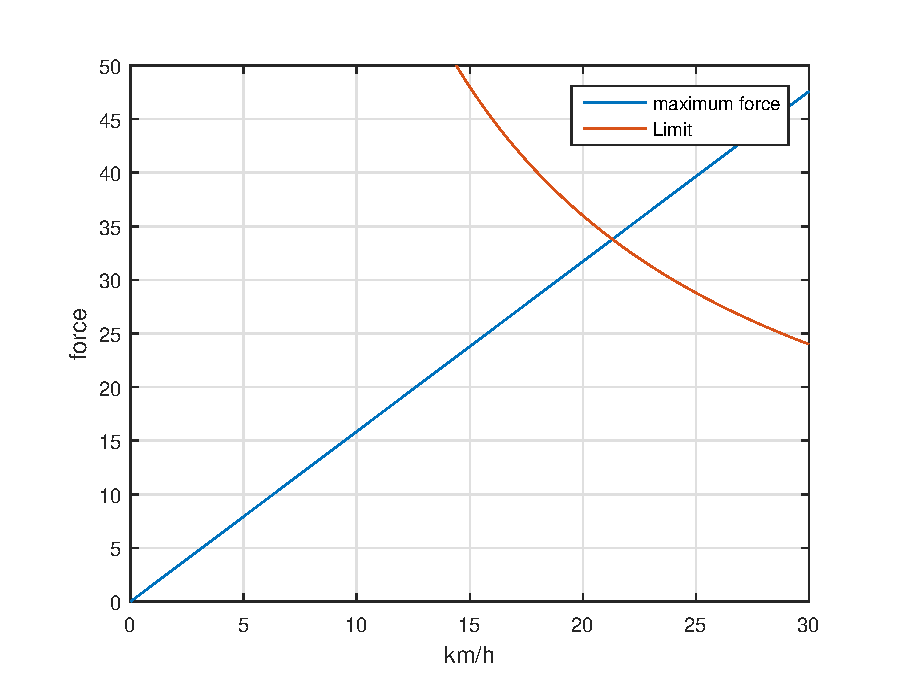
\includegraphics [width=4in]{Hardware/Pictures/force.eps}
	\caption{This diagram give shows how much force that maximum can get from a speed with this setup. The other line shows where 200 W limit is.}
	\label{fig:Force_and_speed}
\end{figure}
\subsection{Super Capacitor}
As explained in the Load System's analysis, in section \vref{sec:LoadSystemAnalysis}, the Generator's internal armature has an inductive reactance. This causes the Generator to resist a sudden change in current which isn't desirable due to the switching application of the MOSFET.

The problem can be solved by placing a Super Capacitor in parallel with the Generator. As the MOSFET turns off the Generator will impede the change and continue to produce current. This current is then used to charge the capacitor. When the MOSFET turns back on, the Generator will once again impede the change and the state of the current production will be inert. The current can then instead be drawn from the charged capacitor.

% Skriv om ting

\textbf{Calculations - Capacitance}\\
The size of the Super capacitor can be found by the largest specified voltage-drop above it - i.e the largest voltage-drop generated by the Generator. According to the Generator's analysis, in section \vref{sec:GeneratorAnalysis}, this voltage is generated at AU2's cruise speed and is equal to:
\begin{equation}
	V_b = \SI{18.16}{\volt}
\end{equation}
 %%
 
The biggest allowed voltage-drop over one switching-period can be calculated as the difference between the two values above:
\begin{equation}
	dV = V_b - V_{b,minimum} = \SI{18.16}{\volt} - \SI{16.13}{\volt} = \SI{2.03}{\volt}
\end{equation}
 
The MOSFET's switchfrequency f\textsubscript{switch} is chosen to be equal to \SI{20}{\kilo \hertz}. The time between each switch can then be calculated as:
\begin{equation}
	dt = \frac{1}{f_{switch}} = \frac{1}{\SI{20}{\kilo \hertz}} = \SI{0.05}{\milli \second}
\end{equation}

The minimum value of the Super Capacitor's capacitance can be found using the capacitor-formula below and the values found above:
\begin{equation}
	\begin{split}
		I &= C \cdot \frac{dV}{dt}\\
		\\
		\SI{13.484}{\ampere} &= C \cdot \frac{\SI{2.03}{\volt}}{\SI{0.05}{\milli \second}} \quad \Rightarrow \quad C = \SI{333}{\micro \farad}
	\end{split}
\end{equation}

The chosen type of super capacitor is a Epcos B41570 Aluminum electrolytic capacitor. This capacitor has a capacitance of \SI{10}{\milli \farad} and is rated to be able to handle a DC-voltage of \SI{100}{\volt}. The chosen capacitor has a much larger value than the one needed. However, this will only cause the voltage-drop dV to be much smaller than the required. The new voltage-drop can be found as:
\begin{equation}
	\begin{split}
		I &= C \cdot \frac{dV}{dt}\\
		\\
	\SI{13.484}{\ampere} &= \SI{10}{\milli \farad} \cdot \frac{dV}{\SI{0.05}{\milli \second}} \quad \Rightarrow \quad dV = \SI{67}{\milli \volt}
	\end{split}
\end{equation}

\textbf{Calculations - Power}\\
Due to the non-ideal nature of the capacitor it will contain both a resistance and a reactance. This means that both an active an a reactive power will be generated in the Super Capacitor. The active power can be calculated using the capacitor's equivalent series resistance (ESR):
\begin{equation}
	P_C = I_{C,rms}^2 \cdot ESR
\end{equation}

Where I\textsubscript{C,rms} is the rms-value of the current in the Super Capacitor. This value will be largest when MOSFET is operating with a duty-cycle of precisely 50\% and the Generator is generating the largest possible voltage. The power in the Load can then be found as:
\begin{equation}
	I_{load} = \frac{V_b}{R_{load}} \cdot 0.50 = \frac{\SI{18.16}{\volt}}{\SI{1.1065}{\ohm}} \cdot 0.50 = \SI{8.255}{\ampere}
\end{equation}

This current will be drawn from the capacitor when the MOSFET is on and the flow back into it when the MOSFET is off. If it is assumed that this change in direction happens instantaneous, then the current in the capacitor over a period T can be described using the following function:
\begin{equation}
	I_c(t) = I_{load} - 2 \cdot I_{load} \cdot u \left( t - \frac{T}{2} \right)
\end{equation}

Where u(t) is the unit-step-function. For a square-waved signal the rms-value can be found as the amplitude of the signal which is \SI{8.255}{\ampere}. Furthermore, the chosen capacitor is rated to have an equivalent series resistance (ESR) of \SI{15}{\milli \ohm}. The active power generated in the capacitor can therefore be calculated as:
\begin{equation}
	P_C = I_{C,rms}^2 \cdot ESR = (\SI{8.255}{\ampere})^2 \cdot \SI{15}{\milli \ohm} = \SI{1.022}{\watt}
\end{equation}

\textbf{Calculations - RCL-filter}\\
The coupling between the Generator and the Super Capacitor creates a low-pass RCL-filter due to the internal impedance in the Generator. The filter is seen below:

\begin{figure}[H]
	\centering
	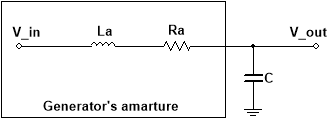
\includegraphics[width=0.5\linewidth]{Hardware/LoadSystem/RLC_filter}
	\caption{RLC-filter consisting of the Generator and the Super Capacitor}
	\label{fig:RLC_filter}
\end{figure}

The filter's transfer function in the s-domain can be found using the Laplace-transform. Using circuit-analysis the function below is found: 
\begin{equation}
	G(s) = \frac{1}{CLs^2 + CRs + 1}
\end{equation}

 The filter's frequency-response as well as the cutoff-frequency can be calculated using the specified values for the capacitance, resistance and the inductance.
\begin{equation}
	\begin{split}
		L_a &= \SI{0.072}{\milli \henry}\\
		R_a &= \SI{103}{\milli \ohm}\\
		C &= \SI{10}{\milli \farad}\\
		\\
		f_c &= \frac{1}{\sqrt{L_a \cdot C}} = \frac{1}{\sqrt{\SI{0.072}{\milli \henry} \cdot \SI{10}{\milli \farad}}} = \SI[per-mode=fraction]{1178}{\radian \per \second} = \SI{187.6}{\hertz}
	\end{split}
\end{equation}

The frequency response is represented below in the form of a Bode-plot.

% bode plot

Using the filter's transfer function it can be found that the amplification at the switching frequency f\textsubscript{switch} of \SI{20}{\kilo \hertz} is equal to \SI{-80}{dB}. At such high damping the the output-signal can effectively be assumed to be a DC-value.

\subsection{Implementation}
Text

\begin{figure}[H]
	\centering
	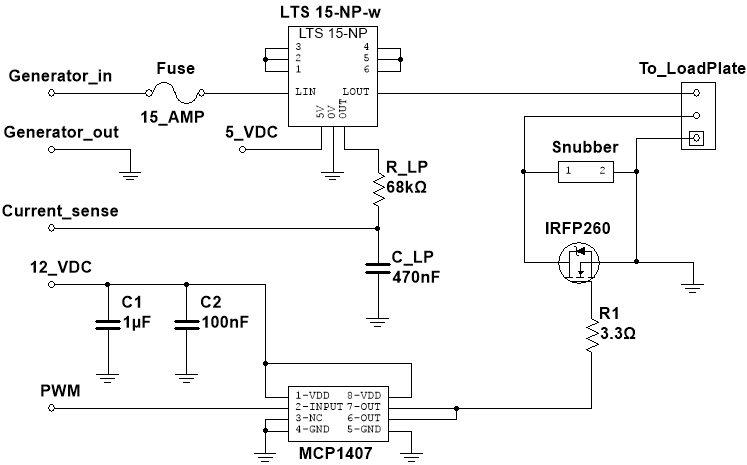
\includegraphics[width=1\linewidth]{Hardware/LoadSystem/LoadSystem}
	\caption{Complete Load System implemented on the Control-box}
	\label{fig:LoadSystemCircuit}
\end{figure}


\subsection{Unity test}
Text